\documentclass[11pt]{article}

%================================================================
%================================================================
%
%                           Preamble
%
%================================================================
%================================================================

%======================================================
%
%                      Packages
%
%======================================================

\usepackage[margin=1in]{geometry}  % set the margins to 1in
\usepackage{graphicx}              % to include figures
\usepackage{amsmath}               % great math stuff
\usepackage{amsfonts}              % for blackboard bold, etc
\usepackage{amsthm}                % better theorem environments
\usepackage{titlesec}              % format section titles

\usepackage{soul}
\usepackage{mathrsfs}
\usepackage{enumerate}
\usepackage{multicol}
\usepackage[makeroom]{cancel}
\usepackage{xcolor}
%\usepackage[usenames,dvipsnames]{color}
\usepackage{tikz}
\usepackage{setspace}
\usepackage{pdfpages}
\usepackage{listings}
\usepackage{matlab-prettifier}
\usepackage{xspace}
\usepackage{multirow}

\usepackage{amssymb}
\usepackage{parskip}
\usepackage{color}
\usepackage[hyphens]{url}
\usepackage{latexsym}
\usepackage{fancyhdr}
\usepackage{fancyvrb}
\usepackage{algpseudocode}
\usepackage{verbatim}
\usepackage{collectbox}
\usepackage{scrextend}
\usepackage{array}
\usetikzlibrary{arrows.meta,shapes,calc}

\DeclareMathOperator{\id}{id}

%======================================================
%
%                   New Commands
%
%======================================================

\newcommand{\bd}[1]{\mathbf{#1}}  % for bolding symbols
\newcommand{\RR}{\mathbb{R}}      % for Real numbers
\newcommand{\ZZ}{\mathbb{Z}}      % for Integers
\newcommand{\col}[1]{\left[\begin{matrix} #1 \end{matrix} \right]}
\newcommand{\comb}[2]{\binom{#1^2 + #2^2}{#1+#2}}
\newcommand{\overfrac}[2]{\genfrac{}{}{0pt}{}{#1}{#2}}

\newcommand{\numdash}{\nobreakdash--}
\newcommand{\blank}[1]{\underline{\hspace{#1}}}
\newcommand{\N}{\ensuremath{\mathbb{N}}}
\newcommand{\Z}{\ensuremath{\mathbb{Z}}}
\newcommand{\Q}{\ensuremath{\mathbb{Q}}}
\newcommand{\R}{\ensuremath{\mathbb{R}}}
\newcommand{\C}{\ensuremath{\mathbb{C}}}
\newcommand{\B}{\ensuremath{\mathbb{B}}}
\newcommand{\T}{\ensuremath{\mathbb{T}}}
\newcommand{\Tau}{\ensuremath{\mathcal{T}}}
\newcommand{\HS}{\ensuremath{\mathcal{H}}}
\newcommand{\intom}{\ensuremath{\int_{\Omega}}}
\newcommand{\fa}{\ensuremath{\ \forall\ }}
\newcommand{\ex}{\ensuremath{\ \exists\ }}
\newcommand{\idty}{{\mathchoice {\rm 1\mskip-4mu l} {\rm 1\mskip-4mu l} %
    {\rm 1\mskip-4.5mu l} {\rm 1\mskip-5mu l}}}
\newcommand{\MATLAB}{\textsc{Matlab}\xspace}
\newcommand{\norm}[1]{\left\lVert#1\right\rVert}

\newtheorem{proposition}{Proposition}[section]
\newtheorem{lemma}[proposition]{Lemma}
\newtheorem{theorem}[proposition]{Theorem}
\newtheorem{corollary}[proposition]{Corollary}
\newtheorem{conjecture}[proposition]{Conjecture}
\theoremstyle{definition}
\newtheorem{definition}[proposition]{Definition}
\newtheorem{example}[proposition]{Example}
\theoremstyle{remark}
\newtheorem{remark}[proposition]{Remark}
\newtheorem{claim}[proposition]{Claim}
\newtheorem{notation}[proposition]{Notation}

\def\Xint#1{\mathchoice
	{\XXint\displaystyle\textstyle{#1}}%
	{\XXint\textstyle\scriptstyle{#1}}%
	{\XXint\scriptstyle\scriptscriptstyle{#1}}%
	{\XXint\scriptscriptstyle\scriptscriptstyle{#1}}%
	\!\int}
\def\XXint#1#2#3{{\setbox0=\hbox{$#1{#2#3}{\int}$ }
		\vcenter{\hbox{$#2#3$ }}\kern-.6\wd0}}
\def\ddashint{\Xint=}
\def\dashint{\Xint-}

\makeatletter
\newcommand{\mybox}{%
	\collectbox{%
		\setlength{\fboxsep}{1pt}%
		\fbox{\BOXCONTENT}%
	}%
}
\makeatother

\newcommand{\newquestion}{\hrulefill\vspace{-0.8\baselineskip}\\\null\hrulefill\vspace{-1.0\baselineskip}}
\newcommand{\newpart}{\vspace{-0.5\baselineskip}\hrulefill\vspace{-1.3\baselineskip}}

\DeclareMathOperator{\ran}{ran}
\DeclareMathOperator{\krnl}{ker}
\DeclareMathOperator{\dist}{dist}
\DeclareMathOperator{\image}{im}
\DeclareMathOperator{\supp}{supp}
\DeclareMathOperator{\vol}{vol}
\DeclareMathOperator{\spn}{span}
\DeclareMathOperator{\GL}{GL}
\DeclareMathOperator{\card}{card}
\DeclareMathOperator{\LCM}{LCM}
\DeclareMathOperator{\HCF}{HCF}

%\numberwithin{equation}{chapter}

%======================================================
%
%                   Format Specifications
%
%======================================================

\everymath{\displaystyle}
\setlength\parindent{0pt}
\titleformat{\section}{\normalfont}{\thesection}{}{}
\titleformat{\subsection}{\normalfont}{\thesubsection}{}{}
\titleformat{\subsubsection}{\normalfont}{\thesubsubsection}{}{}
\theoremstyle{plain}

\lstset{
  numbers=left,
  numberstyle=\scriptsize,
  stepnumber=1,
  numbersep=8pt,
  showstringspaces=false,
  breaklines=true,
  frame=single
}

%================================================================
%================================================================
%
%                          Homework 5
%
%================================================================
%================================================================
\begin{document}
  \begin{flushright}
    Mikhail Gaerlan\\
    16 March 2018\\
    MAT 226B Freund
  \end{flushright}
\vspace{-1.3\baselineskip}

\newquestion
%======================================================
%
%                    Problem 1
%
%======================================================
\section*{Problem 1}
\lstinputlisting[style=Matlab-editor,basicstyle=\ttfamily\small]{../Code/solvePoisson.m}
\lstinputlisting[style=Matlab-editor,basicstyle=\ttfamily\small]{../Code/multAp.m}\newpage
\lstinputlisting[style=Matlab-editor,basicstyle=\ttfamily\small]{../Code/poissonSolve.m}
\lstinputlisting[style=Matlab-editor,basicstyle=\ttfamily\small]{../Code/homework5_1_1.m}
\begin{center}
  \begin{tabular}{c|c|c}
    $\gamma$&Iterations&Relative Residual Norm\\\hline
    $\begin{array}{l}
       1\\
       10\\
       50\\
       100\\
       1000
     \end{array}$
            &$\begin{array}{r}
\texttt{7}\\
\texttt{18}\\
\texttt{50}\\
\texttt{83}\\
\texttt{391}\\
\end{array}
$&$\begin{array}{r}
\texttt{3.877478556473064e-11}\\
\texttt{3.548776304593922e-11}\\
\texttt{8.226758443269179e-11}\\
\texttt{8.780792025563864e-11}\\
\texttt{9.733282686797891e-11}\\
\end{array}
$
  \end{tabular}
\end{center}
\begin{center}
  \begin{tabular}{|c|c|}
    \hline
    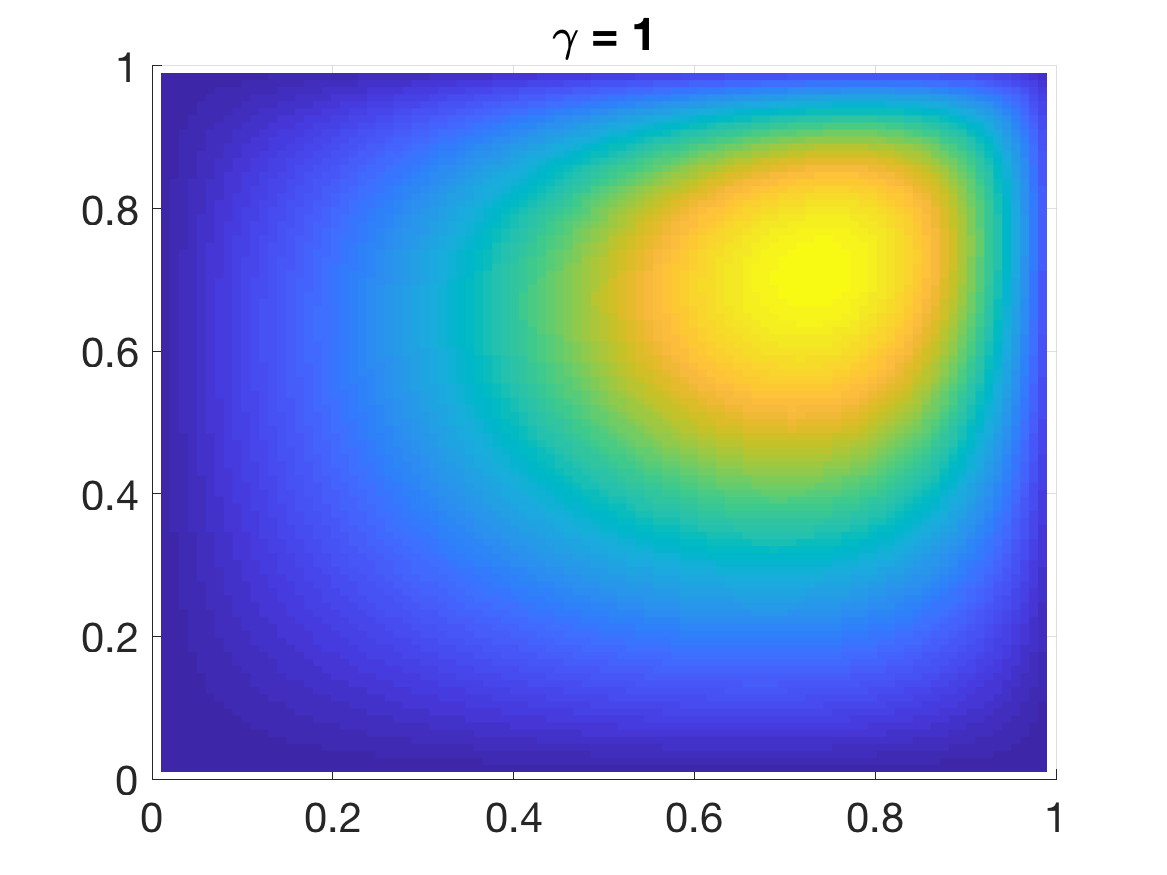
\includegraphics[width=0.45\linewidth]{../Figures/homework5_1_1.png}&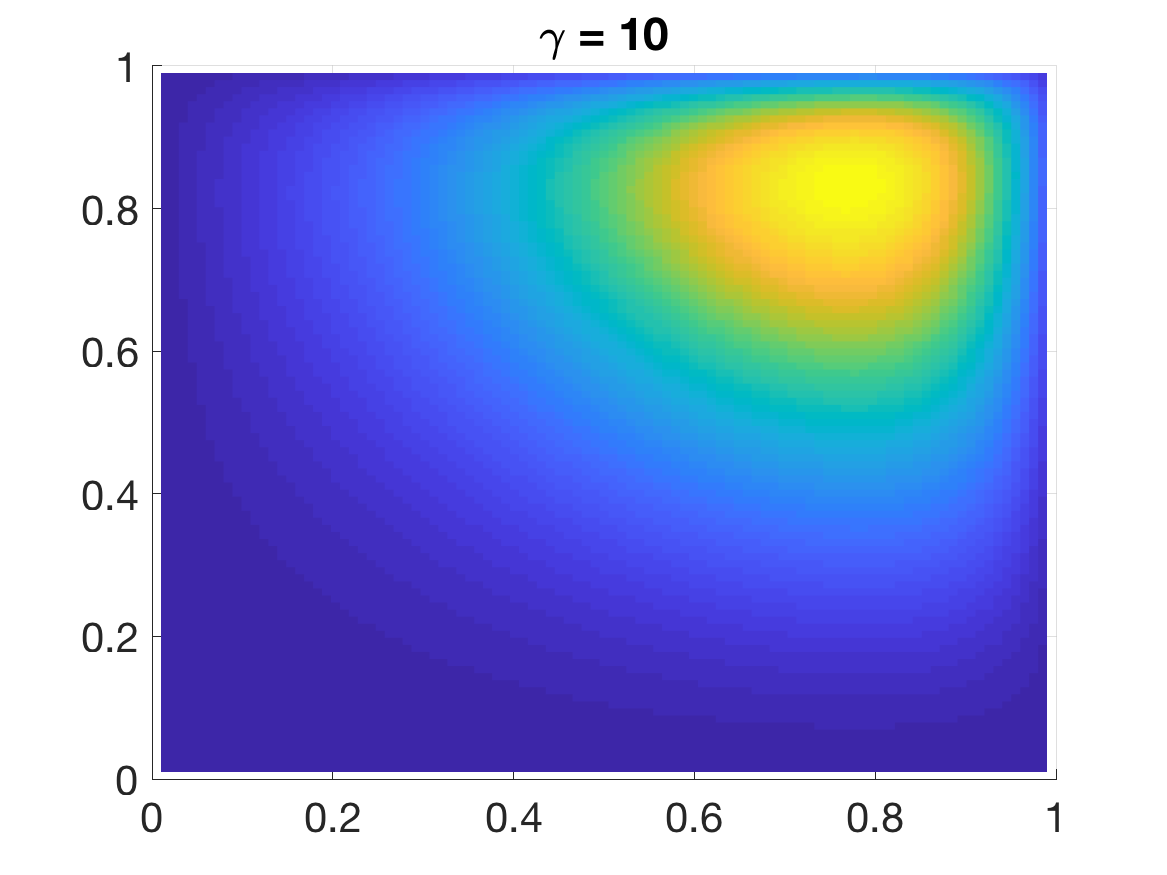
\includegraphics[width=0.45\linewidth]{../Figures/homework5_1_10.png}\\\hline
    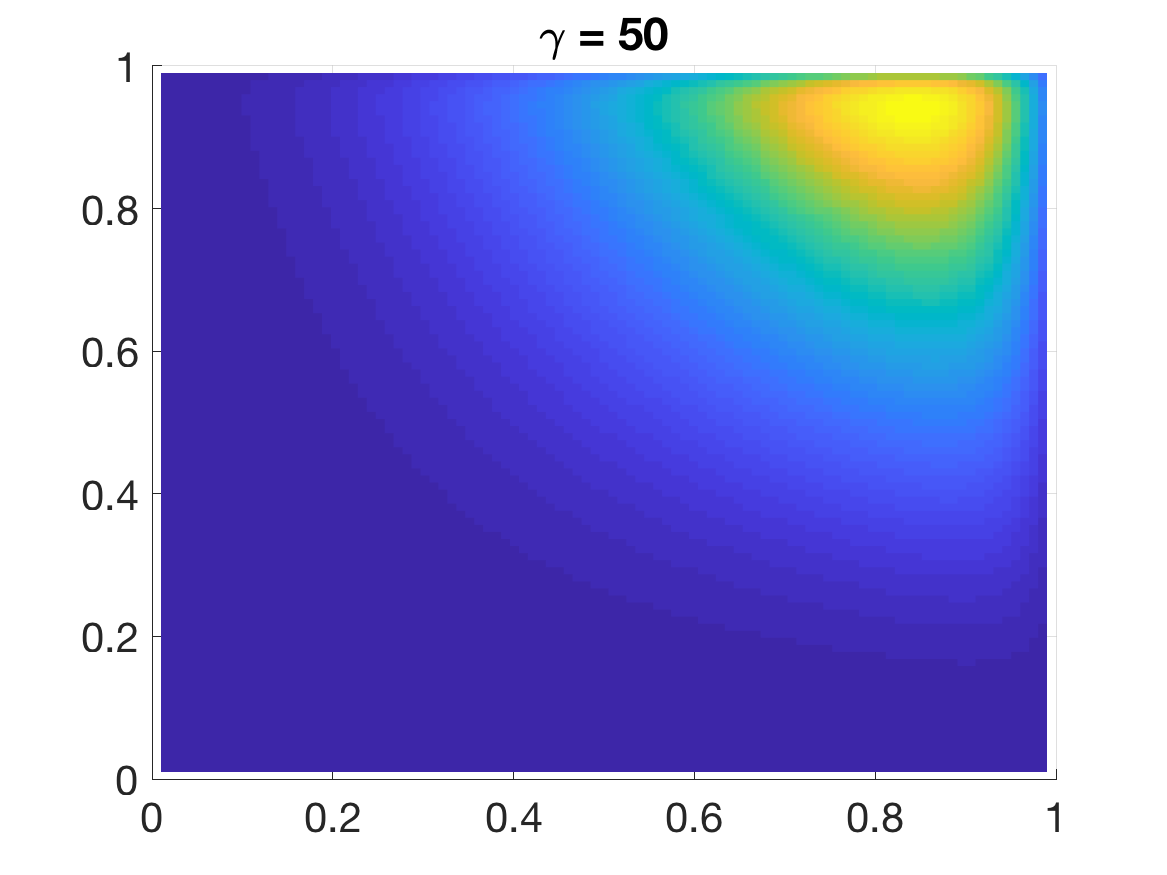
\includegraphics[width=0.45\linewidth]{../Figures/homework5_1_50.png}&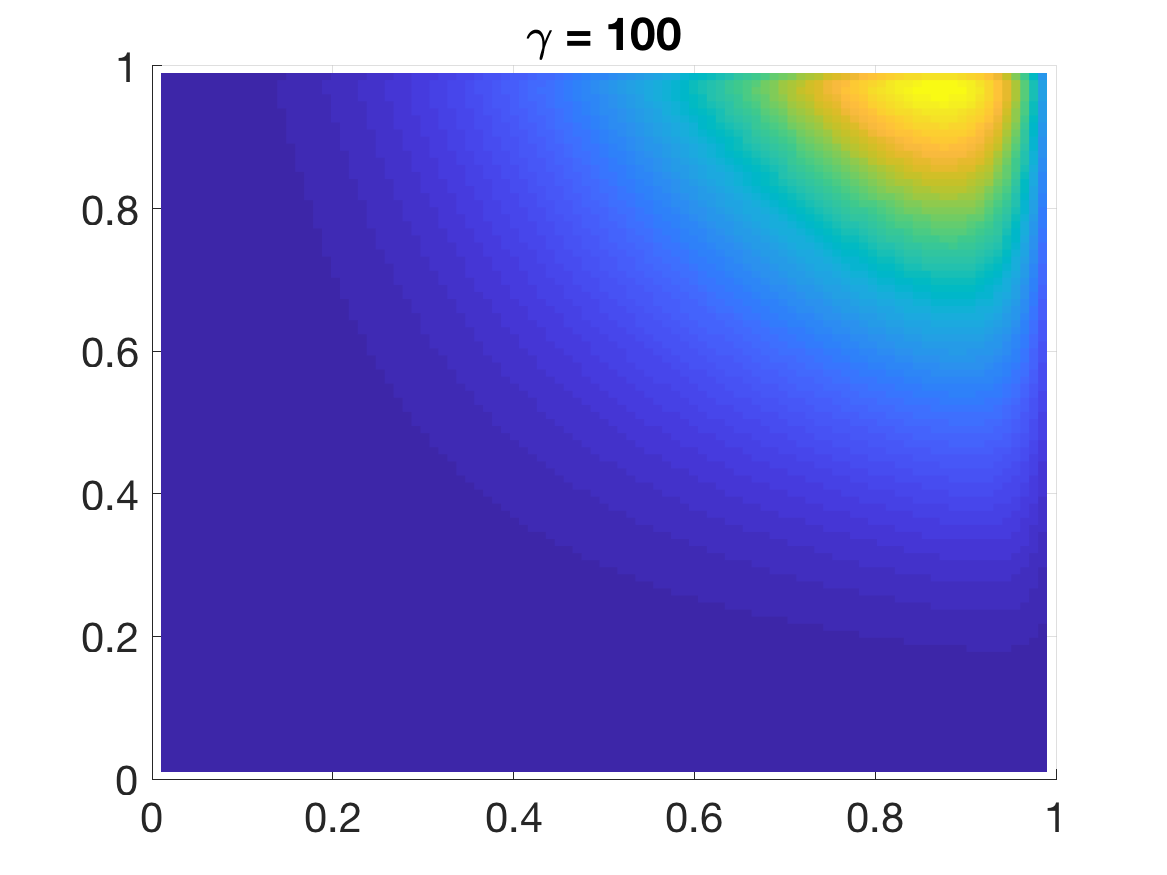
\includegraphics[width=0.45\linewidth]{../Figures/homework5_1_100.png}\\\hline
    \multicolumn{2}{|c|}{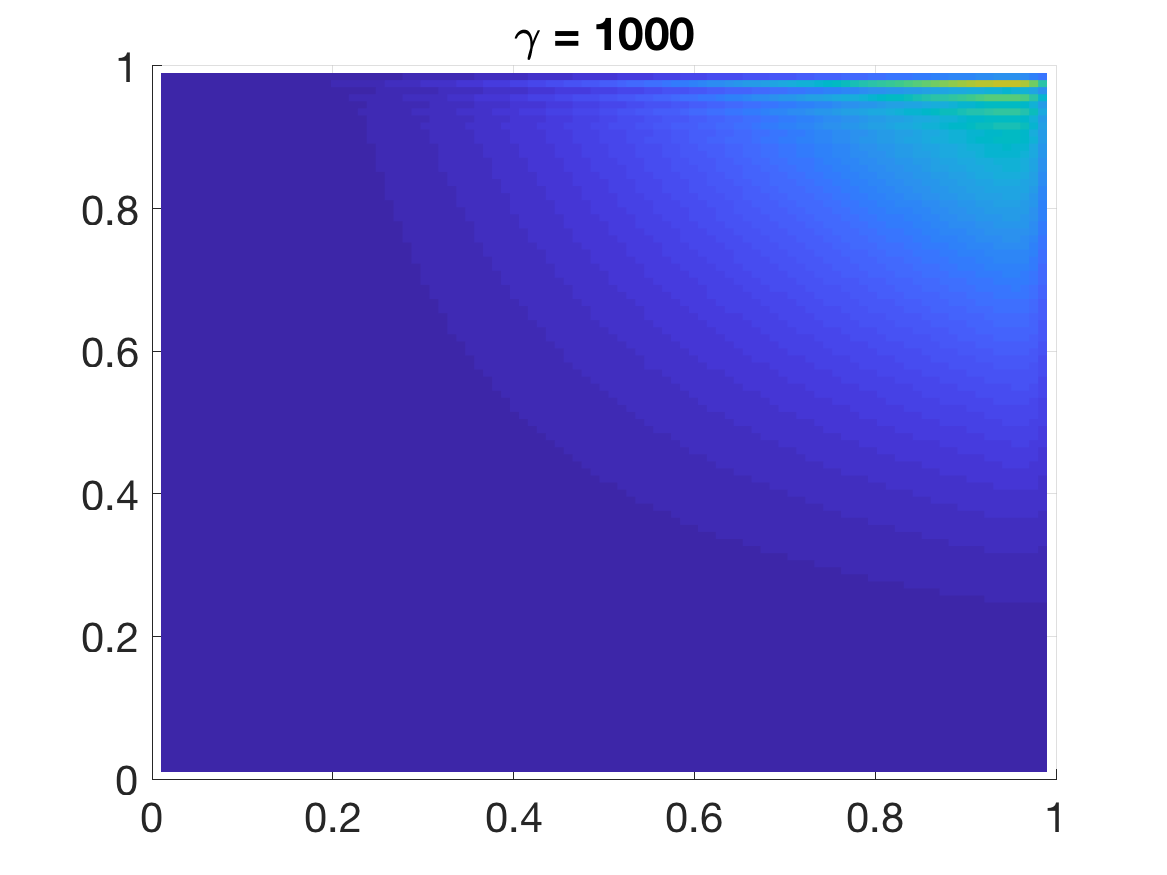
\includegraphics[width=0.45\linewidth]{../Figures/homework5_1_1000.png}}\\\hline
  \end{tabular}
\end{center}\newpage

\newquestion
%======================================================
%
%                    Problem 2
%
%======================================================
\section*{Problem 2}
\begin{eqnarray*}
  x_1^{\textrm{CG}}&=&x_0+\frac{r_0^Tr_0}{r_0^TAr_0}r_0
\end{eqnarray*}
???

\newquestion
%======================================================
%
%                    Problem 3
%
%======================================================
\section*{Problem 3}
With an initial vector $r$, we can use the Hermitian Lanczos process to find an $H_k$ and $V_k$ such that $A\approx V_kH_kV_k^H$. Then
\begin{eqnarray*}
  \left(A\lambda\right)^2&\approx&V_kH_kV_k^H\lambda V_kH_kV_k^H\lambda\\
                         &\approx&V_kH_kV_k^HV_kH_kV_k^H\lambda^2\\
     &\approx&V_kH_kH_kV_k^H\lambda^2\\
     &\approx&V_k\left(H_k\lambda \right)^2V_k^H\\
  A^j&\approx&V_k\left(H_k\lambda\right)^jV_k^H\\
  e^{A\lambda}b&\approx&\left(\sum_{j=0}^\infty\frac{1}{j!}V_k\left(H_k\lambda\right)^jV_k^H\right)b\\
     &\approx&V_k\left(\sum_{j=0}^\infty\frac{1}{j!}\left(H_k\lambda\right)^j\right)V_k^Hb\\
     &\approx&V_ke^{H_k\lambda}V_k^Hb
\end{eqnarray*}
which only requires $k\times k$, $k\times n$, and $n\times k$ matrix multiplications where $k\ll n$.

\newpage
\newquestion
%======================================================
%
%                    Problem 4
%
%======================================================
\section*{Problem 4}
\lstinputlisting[style=Matlab-editor,basicstyle=\ttfamily\small]{../Code/arnoldi.m}
\lstinputlisting[style=Matlab-editor,basicstyle=\ttfamily\small]{../Code/homework5_4_1.m}
\begin{center}
  \begin{tabular}{c|c|c}
    $\gamma$&Iterations&Relative Residual Norm\\\hline
    $\begin{array}{l}
       1\\
       10\\
       50\\
       100\\
       1000
     \end{array}$
            &$\begin{array}{r}
\texttt{0.000000000000000e+00}\\
\texttt{0.000000000000000e+00}\\
\texttt{0.000000000000000e+00}\\
\texttt{0.000000000000000e+00}\\
\texttt{0.000000000000000e+00}\\
\end{array}
$&$\begin{array}{r}
\texttt{1.226016708116490e-01}\\
\texttt{8.580633957899474e-03}\\
\texttt{4.159214697792878e-02}\\
\texttt{7.755234807196754e-02}\\
\texttt{8.129363507071738e-01}\\
\end{array}
$
  \end{tabular}
\end{center}\newpage
\begingroup
\fontsize{8pt}{12pt}\selectfont
\begin{center} $\gamma = 1$ \end{center}
\begin{multicols}{2}
  \begin{tabular}{c}
    $\lambda_j$ such that $j = \underset{1\leq i\leq k}{\textrm{argmin}}\left(\rho_i\right)$\\\hline
    $\begin{array}{r}
\texttt{5.925824662088014e-16}\\
\texttt{-7.169849399663779e-17}\\
\texttt{1.000000000000002e+00+1.124896368980689e-01i}\\
\texttt{1.000000000000002e+00-1.124896368980689e-01i}\\
\end{array}
$
  \end{tabular}
  
  \begin{tabular}{c}
    $\lambda_j$ such that $j = \underset{1\leq i\leq k}{\textrm{argmax}}\left(\rho_i\right)$\\\hline
    $\begin{array}{r}
\texttt{8.613669983806195e-01}\\
\end{array}
$
  \end{tabular}
\end{multicols}
\begin{center} $\gamma = 10$ \end{center}
\begin{multicols}{2}
  \begin{tabular}{c}
    $\lambda_j$ such that $j = \underset{1\leq i\leq k}{\textrm{argmin}}\left(\rho_i\right)$\\\hline
    $\begin{array}{r}
\texttt{1.000000000000003e+00+1.124896368980685e+00i}\\
\texttt{1.000000000000003e+00-1.124896368980685e+00i}\\
\end{array}
$
  \end{tabular}
  
  \begin{tabular}{c}
    $\lambda_j$ such that $j = \underset{1\leq i\leq k}{\textrm{argmax}}\left(\rho_i\right)$\\\hline
    $\begin{array}{r}
\texttt{9.999586452890994e-01+6.220077627914600e-02i}\\
\texttt{9.999586452890994e-01-6.220077627914600e-02i}\\
\end{array}
$
  \end{tabular}
\end{multicols}
\begin{center} $\gamma = 50$ \end{center}
\begin{multicols}{2}
  \begin{tabular}{c}
    $\lambda_j$ such that $j = \underset{1\leq i\leq k}{\textrm{argmin}}\left(\rho_i\right)$\\\hline
    $\begin{array}{r}
\texttt{1.000000000000001e+00+5.624481844903410e+00i}\\
\texttt{1.000000000000001e+00-5.624481844903410e+00i}\\
\texttt{9.999999999999996e-01+3.556289316821839e+00i}\\
\texttt{9.999999999999996e-01-3.556289316821839e+00i}\\
\texttt{1.000000000000000e+00+3.553704482968765e+00i}\\
\texttt{1.000000000000000e+00-3.553704482968765e+00i}\\
\end{array}
$
  \end{tabular}
  
  \begin{tabular}{c}
    $\lambda_j$ such that $j = \underset{1\leq i\leq k}{\textrm{argmax}}\left(\rho_i\right)$\\\hline
    $\begin{array}{r}
\texttt{1.000307573385462e+00+3.092463649917729e-01i}\\
\texttt{1.000307573385462e+00-3.092463649917729e-01i}\\
\end{array}
$
  \end{tabular}
\end{multicols}
\begin{center} $\gamma = 100$ \end{center}
\begin{multicols}{2}
  \begin{tabular}{c}
    $\lambda_j$ such that $j = \underset{1\leq i\leq k}{\textrm{argmin}}\left(\rho_i\right)$\\\hline
    $\begin{array}{r}
\texttt{1.000000000000001e+00+1.124896368980683e+01i}\\
\texttt{1.000000000000001e+00-1.124896368980683e+01i}\\
\texttt{9.999999999999971e-01+7.112578633643686e+00i}\\
\texttt{9.999999999999971e-01-7.112578633643686e+00i}\\
\texttt{1.000000000000004e+00+7.107408965937533e+00i}\\
\texttt{1.000000000000004e+00-7.107408965937533e+00i}\\
\end{array}
$
  \end{tabular}
  
  \begin{tabular}{c}
    $\lambda_j$ such that $j = \underset{1\leq i\leq k}{\textrm{argmax}}\left(\rho_i\right)$\\\hline
    $\begin{array}{r}
\texttt{1.000575887620807e+00+2.346007827840137e-02i}\\
\texttt{1.000575887620807e+00-2.346007827840137e-02i}\\
\end{array}
$
  \end{tabular}
\end{multicols}
\begin{center} $\gamma = 1000$ \end{center}
\begin{multicols}{2}
  \begin{tabular}{c}
    $\lambda_j$ such that $j = \underset{1\leq i\leq k}{\textrm{argmin}}\left(\rho_i\right)$\\\hline
    $\begin{array}{r}
\texttt{1.000000000000009e+00+1.124896368980682e+02i}\\
\texttt{1.000000000000009e+00-1.124896368980682e+02i}\\
\texttt{9.999999999999911e-01+7.112578633643690e+01i}\\
\texttt{9.999999999999911e-01-7.112578633643690e+01i}\\
\texttt{1.000000000000001e+00+7.107408965937532e+01i}\\
\texttt{1.000000000000001e+00-7.107408965937532e+01i}\\
\end{array}
$
  \end{tabular}
  
  \begin{tabular}{c}
    $\lambda_j$ such that $j = \underset{1\leq i\leq k}{\textrm{argmax}}\left(\rho_i\right)$\\\hline
    $\begin{array}{r}
\texttt{9.751427114428090e-01+7.465537420035416e+00i}\\
\texttt{9.751427114428090e-01-7.465537420035416e+00i}\\
\end{array}
$
  \end{tabular}
\end{multicols}
\endgroup
\begin{center}
  \begin{tabular}{|c|c|}
    \hline
    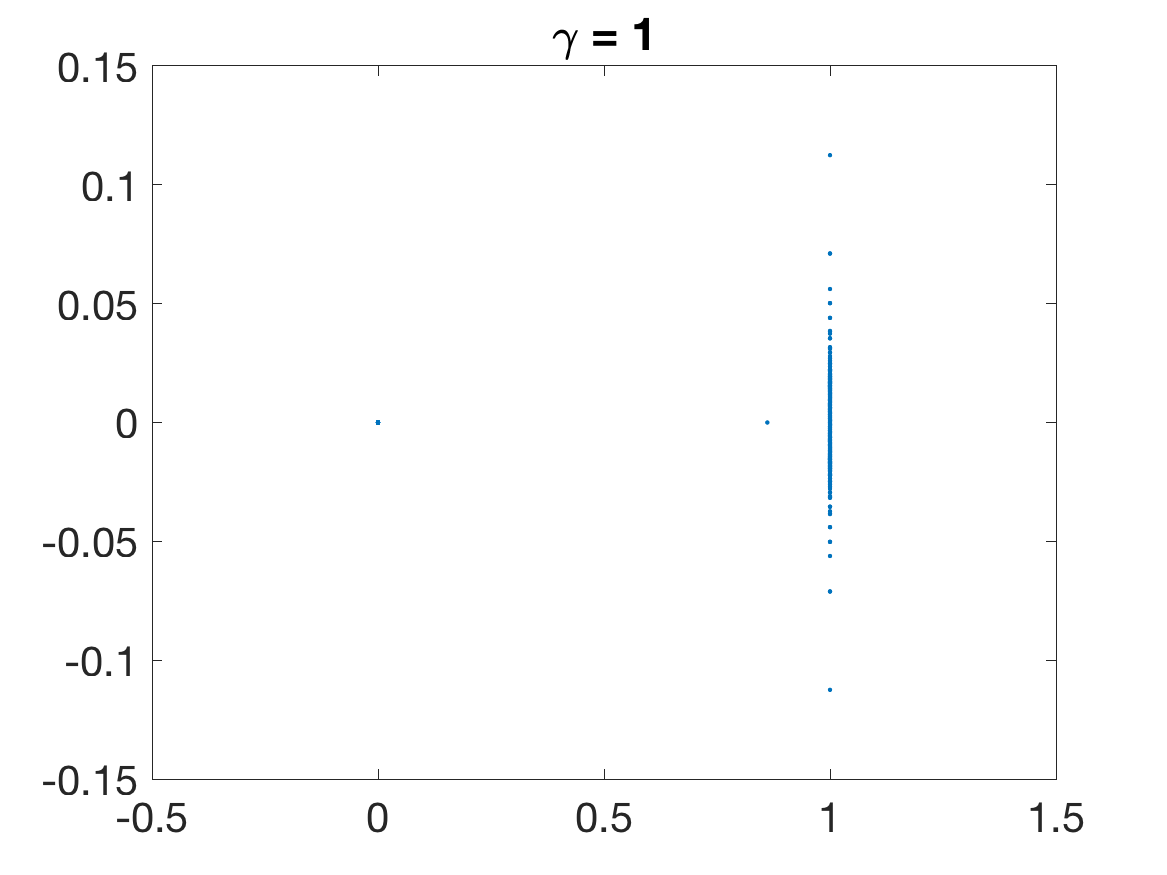
\includegraphics[width=0.45\linewidth]{../Figures/homework5_4_1.png}&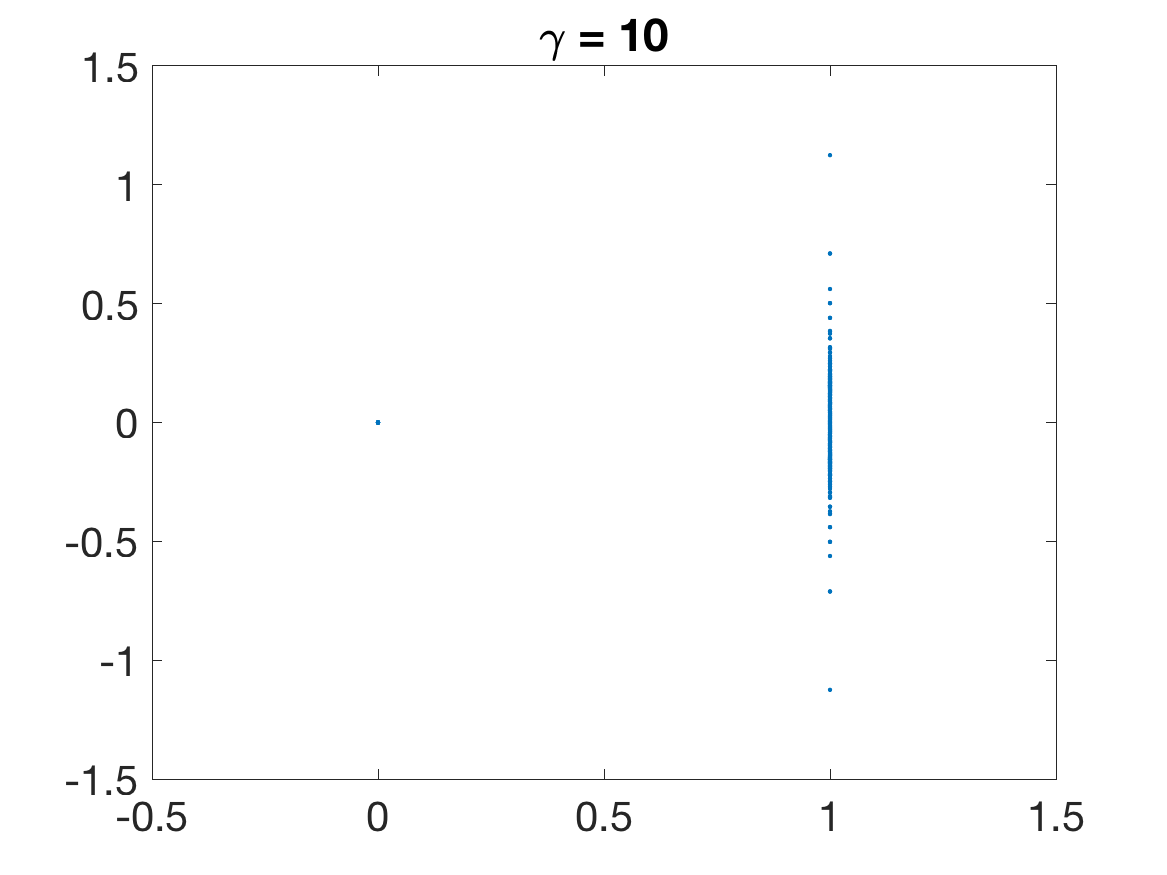
\includegraphics[width=0.45\linewidth]{../Figures/homework5_4_10.png}\\\hline
    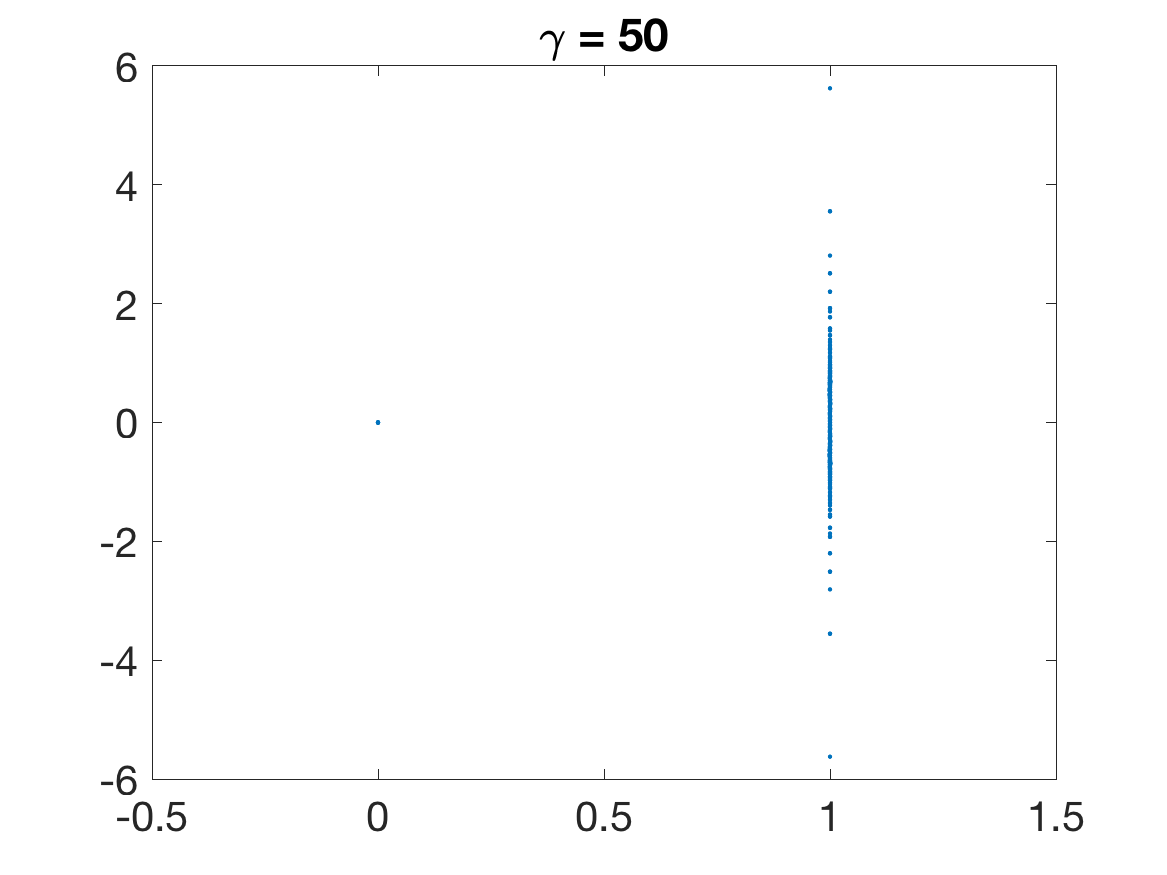
\includegraphics[width=0.45\linewidth]{../Figures/homework5_4_50.png}&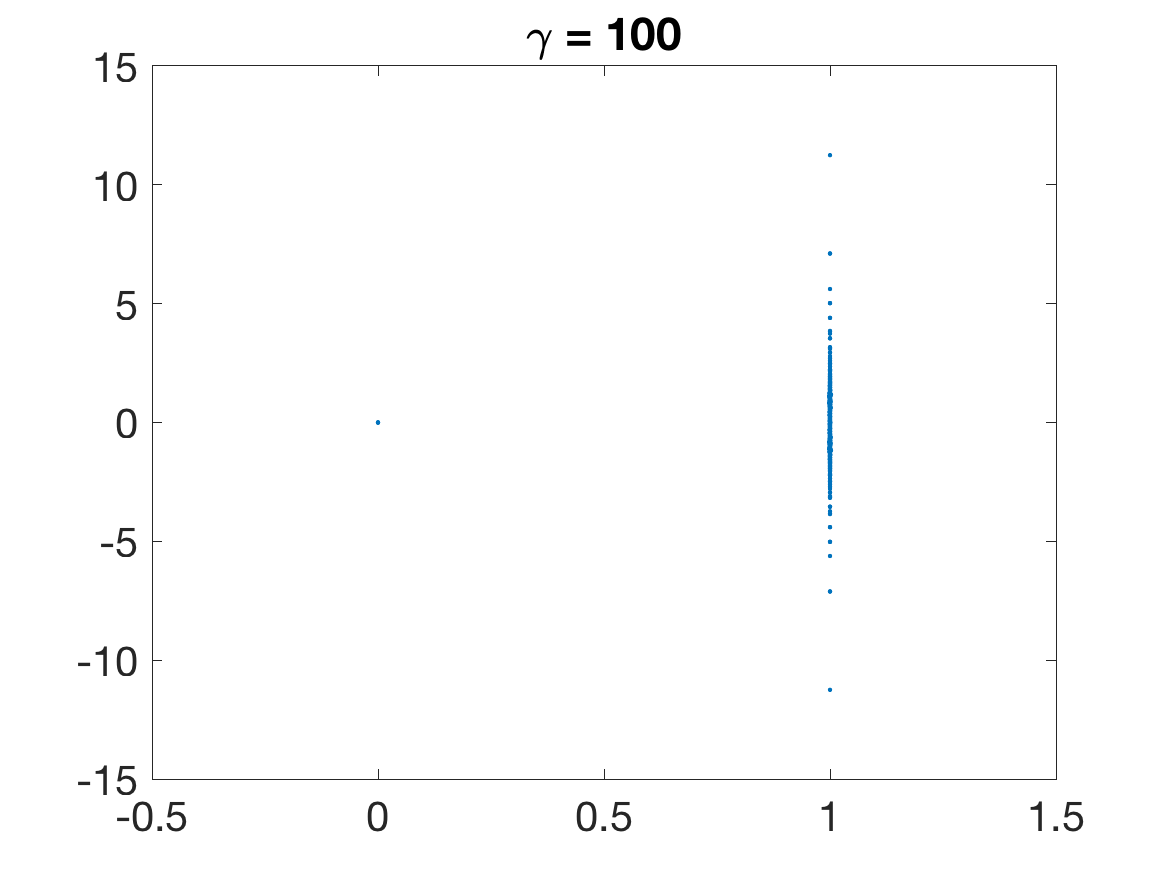
\includegraphics[width=0.45\linewidth]{../Figures/homework5_4_100.png}\\\hline
    \multicolumn{2}{|c|}{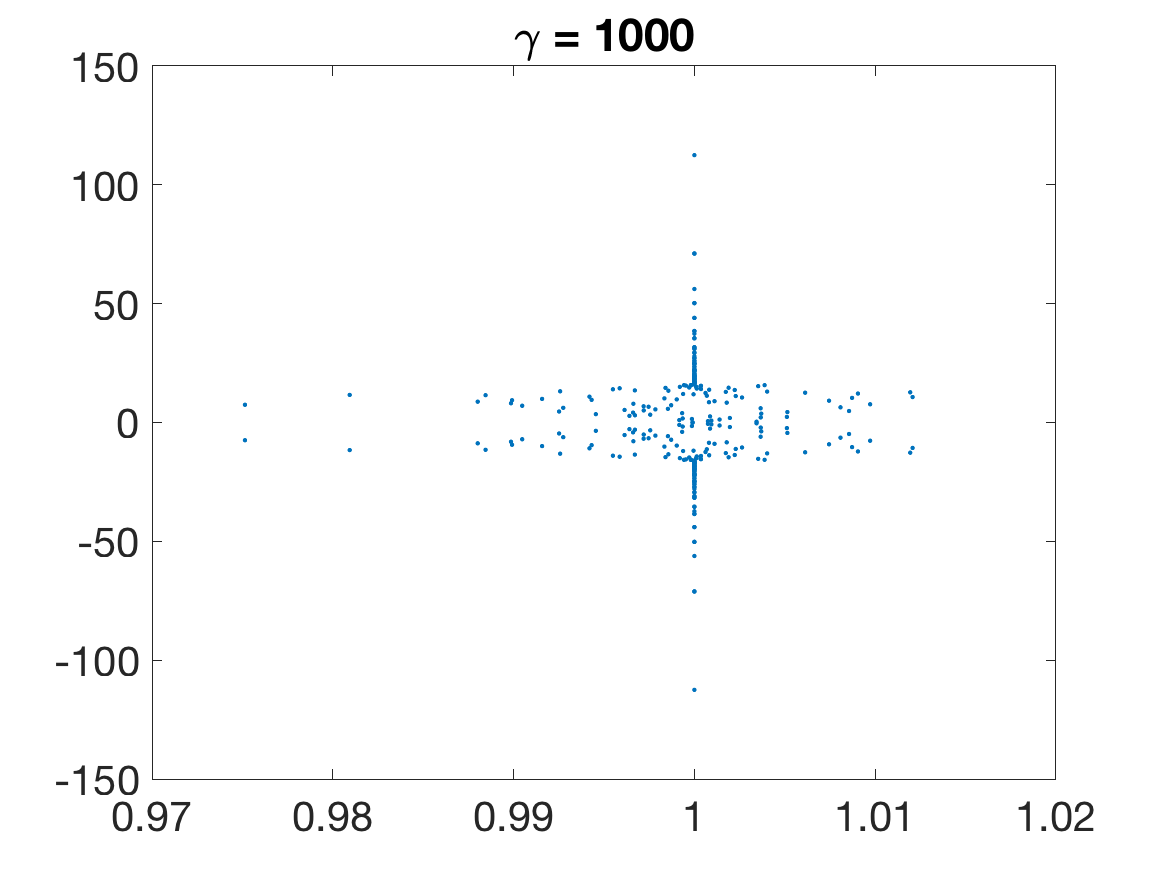
\includegraphics[width=0.45\linewidth]{../Figures/homework5_4_1000.png}}\\\hline
  \end{tabular}
\end{center}\newpage

\newquestion
%======================================================
%
%                    Problem 5
%
%======================================================
\section*{Problem 5}
\lstinputlisting[style=Matlab-editor,basicstyle=\ttfamily\small]{../Code/hermlanc.m}

\newpart
%--------------------------
%    Problem 5 Part A
%--------------------------
\subsection*{(a)}
\lstinputlisting[style=Matlab-editor,basicstyle=\ttfamily\small]{../Code/homework5_5_a_1.m}
\begin{center}
  \begin{tabular}{c|c}
    $\tilde{\lambda}_k$&$\lambda_k$\\\hline
    $\begin{array}{r}
\texttt{3.000000000000000e+00}\\
\texttt{5.000000000000003e+00}\\
\texttt{6.999999999999999e+00}\\
\texttt{9.000000000000002e+00}\\
\end{array}
$&$\begin{array}{r}
\texttt{3.000000000000000e+00}\\
\texttt{5.000000000000000e+00}\\
\texttt{7.000000000000000e+00}\\
\texttt{9.000000000000000e+00}\\
\end{array}
$
  \end{tabular}
\end{center}

\newpage
\newpart
%--------------------------
%    Problem 5 Part B
%--------------------------
\subsection*{(b)}
\lstinputlisting[style=Matlab-editor,basicstyle=\ttfamily\small]{../Code/homework5_5_b_1.m}
\begingroup
\fontsize{8.5pt}{12pt}\selectfont
\begin{center}
  \begin{multicols}{2}
    \begin{tabular}{c|c}
      \multicolumn{2}{c}{$k = 250$ smallest}\\
      $\tilde{\lambda}_k$&$\lambda_k$\\\hline
      $\begin{array}{r}
\texttt{6.041600777348929e-03}\\
\texttt{1.207914596602798e-02}\\
\texttt{1.811677334763728e-02}\\
\texttt{2.213178125207190e-02}\\
\texttt{2.817776082327112e-02}\\
\texttt{3.430388477604603e-02}\\
\texttt{4.073916196053342e-02}\\
\texttt{4.844284495010276e-02}\\
\texttt{5.491496666673977e-02}\\
\texttt{6.427178030291032e-02}\\
\end{array}
$&$\begin{array}{r}
\texttt{6.041600752111798e-03}\\
\texttt{1.207914584426306e-02}\\
\texttt{1.811669093641410e-02}\\
\texttt{2.212821029887158e-02}\\
\texttt{2.415423602856515e-02}\\
\texttt{2.816575539102262e-02}\\
\texttt{3.420330048317366e-02}\\
\texttt{3.616855663748186e-02}\\
\texttt{3.821481984563135e-02}\\
\texttt{4.220610172963291e-02}\\
\end{array}
$
    \end{tabular}
    
    \begin{tabular}{c|c}
      \multicolumn{2}{c}{largest}\\
      $\tilde{\lambda}_k$&$\lambda_k$\\\hline
      $\begin{array}{r}
\texttt{1.199395839789970e+01}\\
\texttt{1.198792085346275e+01}\\
\texttt{1.198186057903147e+01}\\
\texttt{1.197777726554531e+01}\\
\texttt{1.197301741988887e+01}\\
\texttt{1.197046186175222e+01}\\
\texttt{1.196317078231754e+01}\\
\texttt{1.195560060935483e+01}\\
\texttt{1.194813249018734e+01}\\
\texttt{1.193967841648353e+01}\\
\end{array}
$&$\begin{array}{r}
\texttt{1.199395839924789e+01}\\
\texttt{1.198792085415574e+01}\\
\texttt{1.198188330906359e+01}\\
\texttt{1.197787178970113e+01}\\
\texttt{1.197584576397144e+01}\\
\texttt{1.197183424460898e+01}\\
\texttt{1.196579669951683e+01}\\
\texttt{1.196383144336252e+01}\\
\texttt{1.196178518015437e+01}\\
\texttt{1.195779389827037e+01}\\
\end{array}
$
    \end{tabular}
  \end{multicols}
  \begin{multicols}{2}
    \begin{tabular}{c|c}
      \multicolumn{2}{c}{$k = 500$ smallest}\\
      $\tilde{\lambda}_k$&$\lambda_k$\\\hline
      $\begin{array}{r}
\texttt{6.041600752111682e-03}\\
\texttt{1.207914584426521e-02}\\
\texttt{1.811669093641410e-02}\\
\texttt{2.212821029887092e-02}\\
\texttt{2.415423602856659e-02}\\
\texttt{2.816575539102289e-02}\\
\texttt{3.420330048307895e-02}\\
\texttt{3.616855658492681e-02}\\
\texttt{3.821481941474132e-02}\\
\texttt{4.220609548937836e-02}\\
\end{array}
$&$\begin{array}{r}
\texttt{6.041600752111798e-03}\\
\texttt{1.207914584426306e-02}\\
\texttt{1.811669093641410e-02}\\
\texttt{2.212821029887158e-02}\\
\texttt{2.415423602856515e-02}\\
\texttt{2.816575539102262e-02}\\
\texttt{3.420330048317366e-02}\\
\texttt{3.616855663748186e-02}\\
\texttt{3.821481984563135e-02}\\
\texttt{4.220610172963291e-02}\\
\end{array}
$
    \end{tabular}
    
    \begin{tabular}{c|c}
      \multicolumn{2}{c}{largest}\\
      $\tilde{\lambda}_k$&$\lambda_k$\\\hline
      $\begin{array}{r}
\texttt{1.199395839924789e+01}\\
\texttt{1.198792085415574e+01}\\
\texttt{1.198188330906359e+01}\\
\texttt{1.197787178970113e+01}\\
\texttt{1.197584576397144e+01}\\
\texttt{1.197183424460897e+01}\\
\texttt{1.196579669952040e+01}\\
\texttt{1.196383144337132e+01}\\
\texttt{1.196178518246027e+01}\\
\texttt{1.195779390071517e+01}\\
\end{array}
$&$\begin{array}{r}
\texttt{1.199395839924789e+01}\\
\texttt{1.198792085415574e+01}\\
\texttt{1.198188330906359e+01}\\
\texttt{1.197787178970113e+01}\\
\texttt{1.197584576397144e+01}\\
\texttt{1.197183424460898e+01}\\
\texttt{1.196579669951683e+01}\\
\texttt{1.196383144336252e+01}\\
\texttt{1.196178518015437e+01}\\
\texttt{1.195779389827037e+01}\\
\end{array}
$
    \end{tabular}
  \end{multicols}
  \newpage
  \begin{multicols}{2}
    \begin{tabular}{c|c}
      \multicolumn{2}{c}{$k = 1000$ smallest}\\
      $\tilde{\lambda}_k$&$\lambda_k$\\\hline
      $\begin{array}{r}
\texttt{6.041600752106037e-03}\\
\texttt{6.041600752113144e-03}\\
\texttt{6.041600752114275e-03}\\
\texttt{1.207914584426428e-02}\\
\texttt{1.207914584426578e-02}\\
\texttt{1.211821679530226e-02}\\
\texttt{1.811669093641226e-02}\\
\texttt{1.811669093641471e-02}\\
\texttt{2.212821029887353e-02}\\
\texttt{2.212821029887629e-02}\\
\end{array}
$&$\begin{array}{r}
\texttt{6.041600752111798e-03}\\
\texttt{1.207914584426306e-02}\\
\texttt{1.811669093641410e-02}\\
\texttt{2.212821029887158e-02}\\
\texttt{2.415423602856515e-02}\\
\texttt{2.816575539102262e-02}\\
\texttt{3.420330048317366e-02}\\
\texttt{3.616855663748186e-02}\\
\texttt{3.821481984563135e-02}\\
\texttt{4.220610172963291e-02}\\
\end{array}
$
    \end{tabular}
    
    \begin{tabular}{c|c}
      \multicolumn{2}{c}{largest}\\
      $\tilde{\lambda}_k$&$\lambda_k$\\\hline
      $\begin{array}{r}
\texttt{1.199395839924790e+01}\\
\texttt{1.199395839924789e+01}\\
\texttt{1.199395839924786e+01}\\
\texttt{1.198792085415574e+01}\\
\texttt{1.198792085415573e+01}\\
\texttt{1.198791372575761e+01}\\
\texttt{1.198188330906359e+01}\\
\texttt{1.198188330906359e+01}\\
\texttt{1.197787178970113e+01}\\
\texttt{1.197787178970112e+01}\\
\end{array}
$&$\begin{array}{r}
\texttt{1.199395839924789e+01}\\
\texttt{1.198792085415574e+01}\\
\texttt{1.198188330906359e+01}\\
\texttt{1.197787178970113e+01}\\
\texttt{1.197584576397144e+01}\\
\texttt{1.197183424460898e+01}\\
\texttt{1.196579669951683e+01}\\
\texttt{1.196383144336252e+01}\\
\texttt{1.196178518015437e+01}\\
\texttt{1.195779389827037e+01}\\
\end{array}
$
    \end{tabular}
  \end{multicols}
  \begin{multicols}{2}
    \begin{tabular}{c|c}
      \multicolumn{2}{c}{$k = 2000$ smallest}\\
      $\tilde{\lambda}_k$&$\lambda_k$\\\hline
      $\begin{array}{r}
\texttt{6.041600752108586e-03}\\
\texttt{6.041600752108720e-03}\\
\texttt{6.041600752109451e-03}\\
\texttt{6.041600752112014e-03}\\
\texttt{6.041600752115364e-03}\\
\texttt{6.041602417087011e-03}\\
\texttt{1.207914584424712e-02}\\
\texttt{1.207914584426266e-02}\\
\texttt{1.207914584426319e-02}\\
\texttt{1.207914584426506e-02}\\
\end{array}
$&$\begin{array}{r}
\texttt{6.041600752111798e-03}\\
\texttt{1.207914584426306e-02}\\
\texttt{1.811669093641410e-02}\\
\texttt{2.212821029887158e-02}\\
\texttt{2.415423602856515e-02}\\
\texttt{2.816575539102262e-02}\\
\texttt{3.420330048317366e-02}\\
\texttt{3.616855663748186e-02}\\
\texttt{3.821481984563135e-02}\\
\texttt{4.220610172963291e-02}\\
\end{array}
$
    \end{tabular}
    
    \begin{tabular}{c|c}
      \multicolumn{2}{c}{largest}\\
      $\tilde{\lambda}_k$&$\lambda_k$\\\hline
      $\begin{array}{r}
\texttt{1.199395839924791e+01}\\
\texttt{1.199395839924791e+01}\\
\texttt{1.199395839924788e+01}\\
\texttt{1.199395839924788e+01}\\
\texttt{1.199395839924787e+01}\\
\texttt{1.199395839911458e+01}\\
\texttt{1.198792085415576e+01}\\
\texttt{1.198792085415573e+01}\\
\texttt{1.198792085415573e+01}\\
\texttt{1.198792085415573e+01}\\
\end{array}
$&$\begin{array}{r}
\texttt{1.199395839924789e+01}\\
\texttt{1.198792085415574e+01}\\
\texttt{1.198188330906359e+01}\\
\texttt{1.197787178970113e+01}\\
\texttt{1.197584576397144e+01}\\
\texttt{1.197183424460898e+01}\\
\texttt{1.196579669951683e+01}\\
\texttt{1.196383144336252e+01}\\
\texttt{1.196178518015437e+01}\\
\texttt{1.195779389827037e+01}\\
\end{array}
$
    \end{tabular}
  \end{multicols}
\end{center}
\endgroup

Depending on the value of $k$, the multiplicity of the eigenvalues will change. However, the accruacy of the smallest and largest values seems to not change much based on the value of $k$.

\end{document}
%================================================================
%================================================================
%
%                           Templates
%
%================================================================
%================================================================


%----------------------------------------------------------------
%----------------------------------------------------------------

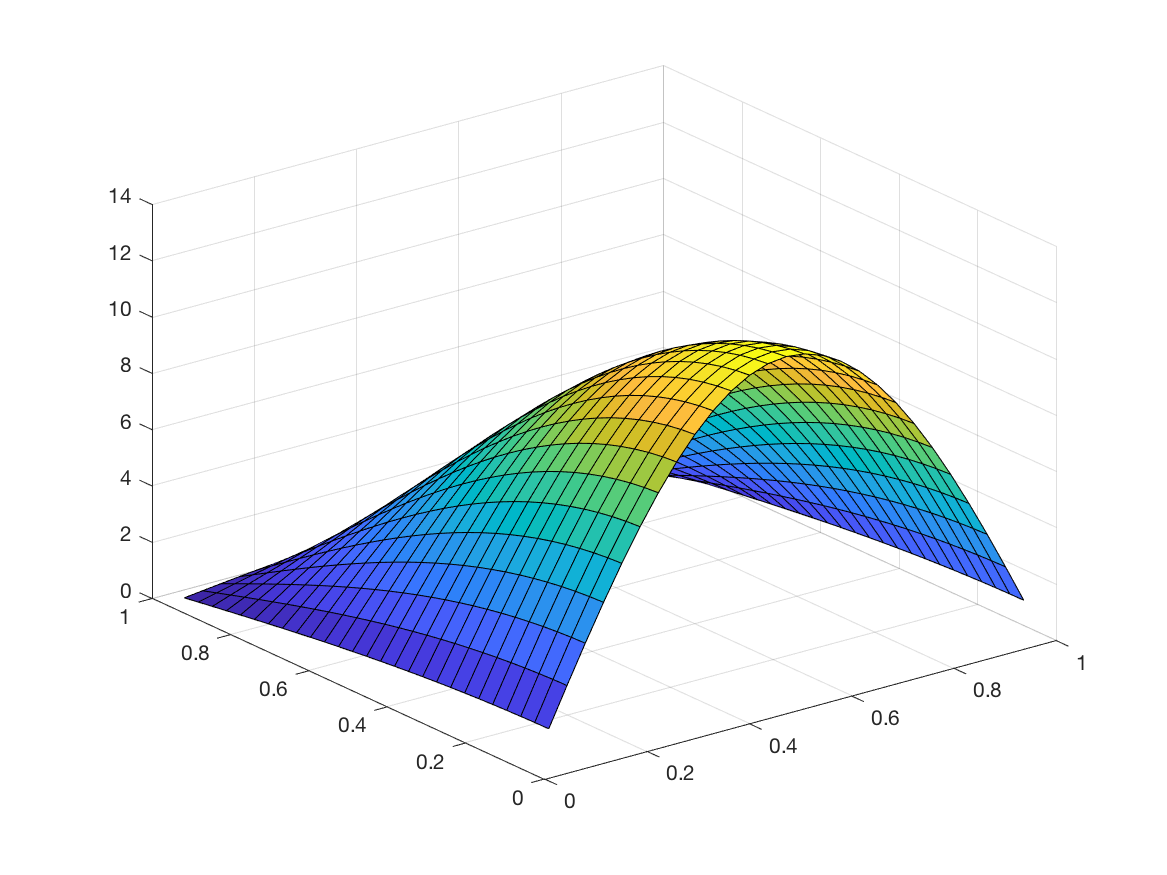
\includegraphics[width=\linewidth]{../Figures/poisson_rhs_1.png}
\lstinputlisting[style=Matlab-editor,basicstyle=\ttfamily\small]{../Code/solvePoisson.m}

\newquestion
%======================================================
%
%                    Problem n
%
%======================================================
\section*{Problem n}

\newpart
%--------------------------
%    Problem n Part A
%--------------------------
\subsection*{(a)}

\newpart
%--------------------------
%    Problem n Part B
%--------------------------
\subsection*{(b)}


%----------------------------------------------------------------
%----------------------------------------------------------------


%======================================================
%
%               Appendix: Problem n
%
%======================================================
%--------------------------
%  Appendix: P n Part A
%--------------------------
\subsection*{Problem n Part A}

\newpage
%--------------------------
%  Appendix: P n Part B
%--------------------------
\subsection*{Problem n Part B}


%----------------------------------------------------------------
%----------------------------------------------------------------